

\ifdefined\maindoc
% Do nothing (we are inside main.tex)
\else
\documentclass[12pt]{report}
\usepackage[a4paper,margin=1in]{geometry}
\usepackage[utf8]{inputenc}
\usepackage[T1]{fontenc}
\usepackage{amsmath,amssymb,amsthm}
\usepackage{booktabs}
\usepackage{setspace}
\usepackage{graphicx}
\usepackage{subcaption}
\usepackage{enumitem}
\usepackage{placeins}
\usepackage{hyperref}
\usepackage{array}
\usepackage{makecell}
\usepackage[backend=biber,style=ieee,citestyle=numeric-comp,sorting=none]{biblatex}
\addbibresource{../../references.bib}
\newtheorem{theorem}{Theorem}
\newtheorem{lemma}[theorem]{Lemma}
\newtheorem{definition}[theorem]{Definition}
\newtheorem{proposition}[theorem]{Proposition}
\onehalfspacing
\graphicspath{{figures/}}
% Standalone-only fallbacks so Chapter~\ref{...} renders as the right number outside the
% main thesis. Under \maindoc these are skipped and the real labels in main.tex resolve.
\makeatletter
\newlabel{ch:system-model}{{3}{1}{}{Doc-Start}{}}
\newlabel{ch:input-module}{{4}{1}{}{Doc-Start}{}}
\newlabel{ch:diamond-module}{{5}{1}{}{Doc-Start}{}}
\makeatother
\begin{document}
\title{Information As Probabilities: Probability Propagation Toolkit}
\fi

\providecommand{\Pa}{\mathrm{Pa}}
\providecommand{\anc}{\mathrm{anc}}
\providecommand{\infl}{\mathrm{infl}}



\section{Introduction}
\label{sec:pp-intro}

Under the probabilistic reading of the network model, the value on a node is the probability that the component operates and the value on an edge the probability that the handover between its endpoints succeeds. The question this reading makes precise is whether information survives the network: with what probability is each node reached from the sources despite component and handover failures. The Probability Propagation Toolkit answers that question exactly, for every node of the network at once, and its propagation algorithm is the framework's namesake, the Information Propagation Algorithm.

The toolkit consumes the unified graph object of Chapter~\ref{ch:input-module} and, wherever the network reconverges, the decomposition structure of Chapter~\ref{ch:diamond-module}. It is the analysis the decomposition module was built for, because reconvergent paths are precisely where local probability calculations stop being valid. Chapter~\ref{ch:diamond-module} surveyed decomposition as a structural strategy. The concern here is the probability computation itself, and a short account of how that computation has been attempted places the toolkit among its alternatives.

\subsection{Computing network reliability}
\label{sec:pp-survey}

The earliest reliability formulations are structural. A reliability block diagram arranges components in series, parallel, and $k$-out-of-$n$ groups whose system reliability has a closed form \cite{billinton1992network}, which is efficient exactly as far as the system is built from those groups. A network whose routes diverge and reconverge with shared upstream components is not, so the redundancy that motivates the analysis is the structure the formalism cannot hold. Fault and event trees widen the reachable logic by building the failure mechanism explicitly as a tree of gates \cite{xing2008fault}, at the price of manual construction and logical expressions that grow rapidly with the number of interacting pathways, and the tree is a model of one failure event rather than of the network, so every source-to-node question needs its own tree.

Graph-theoretic methods compute on the network directly. The reliability of reaching a node is the probability of a union of path events, so minimal path and cut sets, suitably disjointed, give exact answers, and recursive decomposition methods improve on raw enumeration by splitting the network into subproblems \cite{liu2012improved,kim2013network}. Their shared difficulty is that path and cut collections grow combinatorially with exactly the redundancy and reconvergence that make the analysis worth doing. Monte Carlo simulation escapes structure entirely and handles arbitrary networks with confidence intervals in exchange for exactness, with sample counts that grow demanding when failures are rare or answers must be tight \cite{fishman1986comparison}.

Binary decision diagrams brought a different discipline to the exact computation \cite{bryant1986graph,rauzy1993new}. Shannon decomposition compiles the Boolean structure function into a canonical decision graph on which reliability is a single traversal, and the approach handles systems with thousands of variables. Its cost is concentrated in the diagram's size, which depends critically on the variable ordering, and finding a good ordering is itself intractable in general \cite{bryant2002ordered}. Reconvergent fan-out is the diagram's hard case, forcing intermediate nodes to remember which shared ancestors have been decided, and on densely reconvergent networks the construction can exhaust memory under one ordering while remaining compact under another.

The probabilistic-inference literature reaches the same problem from another side. Source-to-node reachability is marginal inference on a directed graphical model, and the exact inference methods are conditioning and clustering: cutset conditioning enumerates the states of a node set whose fixing renders the rest of the structure singly connected \cite{pearl1988probabilistic}, and the junction-tree algorithm clusters the network into a tree of overlapping bags \cite{lauritzen1988local}. Both are exact and both cost exponential in a structural width of the graph, the cutset size for one and the treewidth for the other. Message passing makes the same inference local and scalable when exactness is relaxed, and reliability-specific variants such as the directed probability propagation method track marginal and pairwise probabilities to approximate the dependency structure \cite{tong2019probability}, gaining scale at the price of approximation error and pairwise bookkeeping that grows with the dependent interactions.

One limitation runs across every exact method above: all of them consume point-valued component reliabilities. In practice failure probabilities are estimated from sparse data, elicited from experts, or quoted as manufacturer bounds, and the literature on imprecise probability represents such knowledge as intervals or as probability boxes \cite{ferson2003constructing,williamson1990probabilistic}, bounds on the distribution of the uncertain quantity. None of the exact machinery propagates these forms natively. An interval query against a decision diagram means re-evaluating at chosen input corners, and no analytic route to a distributional bound exists at all.

The toolkit of this chapter is message passing kept exact. Local closed-form updates carry the computation wherever the structure is independent, every reconvergence is resolved by conditioning on the diamonds Chapter~\ref{ch:diamond-module} identified, and solved diamonds reduce to single equivalent components so that no dependence is ever paid for twice. The cost of exactness lands in the same width-governed class as the decision diagram and the junction tree, which Section~\ref{sec:pp-complexity} makes precise and measures. What separates the toolkit from that class is the gap just named: one propagation mechanism, generic over the three value forms of Chapter~\ref{ch:input-module}, returning exact beliefs for point inputs, exact ranges for interval inputs, and guaranteed distributional bounds for probability boxes.

\section{The Belief of a Node}
\label{sec:pp-belief}

Every component of the network can fail. A node $v$ carries its prior $\pi_v$, the probability that the component operates, and an edge $(u,v)$ carries its probability $\rho_{uv}$, the probability that the handover from $u$ to $v$ succeeds, both attached to the graph object during input processing. Writing $X_v$ and $Y_{uv}$ for the corresponding indicator variables, the independence assumption of Chapter~\ref{ch:system-model} makes all of them mutually independent.

Information reaches a node when some path delivers it, and whether it does is itself an indicator variable. The reachability of $v$ is
\begin{equation}
\label{eq:pp-indicator}
R_v \;=\; X_v \,\wedge\, \Bigl(\, v \in S \;\vee\; \bigvee_{u \in \Pa(v)} \bigl( R_u \wedge Y_{uv} \bigr) \Bigr),
\end{equation}
where $S$ is the source set and $\Pa(v)$ the parents of $v$. The toolkit computes the \emph{belief} of every node,
\begin{equation}
\label{eq:pp-belief}
b(v) \;=\; P(R_v = 1),
\end{equation}
the probability that $v$ operates and is reached from at least one source. Unrolling the recursion writes $R_v$ as a disjunction over all source-to-$v$ paths of the conjunction of each path's node and edge indicators, so the belief is equally the probability that at least one path is viable end to end.

Two properties of this quantity govern the whole chapter. Computing $b(v)$ subsumes two-terminal network reliability and is therefore \#P-hard \cite{valiant1979complexity,ball1986computational}, so no exact method escapes exponential cost on every network, and the realistic aim is exactness at a cost set by the structure of the particular network rather than by its size. The second property is that $R_v$ is a monotone Boolean function of the component indicators, since restoring a failed component can only create source-to-node connectivity, never destroy it.

\begin{proposition}[Monotonicity]
\label{prop:pp-monotone}
$b(v)$ is non-decreasing in every node prior and every edge probability.
\end{proposition}

\begin{proof}
Realise each indicator from its own independent uniform variable, $X_w = \mathbf{1}\{U_w \le \pi_w\}$ and $Y_{uw} = \mathbf{1}\{U_{uw} \le \rho_{uw}\}$. Raising any single $\pi_w$ or $\rho_{uw}$ can switch its indicator from $0$ to $1$ but never from $1$ to $0$, and $R_v$ is monotone in every indicator, so on every realisation $R_v$ can only switch from $0$ to $1$. Hence $P(R_v = 1)$ cannot decrease.
\end{proof}

\section{Propagation in a Single Pass}
\label{sec:pp-pass}

A source is reached exactly when it operates, so its belief is its prior. Every other node receives information through its parents. The \emph{signal} through a parent $p$ of $v$ is the event $A_p$ that a viable path reaches $p$ and the handover to $v$ succeeds, with probability
\begin{equation}
\label{eq:pp-signal}
S_p \;=\; b(p)\,\rho_{pv},
\end{equation}
and $v$ is reached when at least one signal arrives, so
\begin{equation}
\label{eq:pp-union}
b(v) \;=\; \pi_v \, P\Bigl(\bigcup_{p \in \Pa(v)} A_p\Bigr).
\end{equation}
When the signal events are mutually independent the union has the closed form
\begin{equation}
\label{eq:pp-independent}
b(v) \;=\; \pi_v \Bigl( 1 - \prod_{p \in \Pa(v)} \bigl( 1 - b(p)\,\rho_{pv} \bigr) \Bigr),
\end{equation}
which for a single parent collapses to the chain rule $b(v) = \pi_v\, b(p)\, \rho_{pv}$.

The iteration sets of Chapter~\ref{ch:input-module} order the computation so that every parent's belief exists before it is consumed. The algorithm initialises the sources, then processes each layer in turn, applying the local update once per node, and Chapter~\ref{ch:input-module}'s convergence guarantee makes the single forward pass complete in exactly $|L|$ layer steps. There is no iterative refinement to converge and no sampling to average, because every update is an exact probability calculation.

Equation~\eqref{eq:pp-independent} evaluates the union as a product of complements rather than by the alternating inclusion-exclusion sum. Under independence the two are identical, but in the product form each signal probability occurs exactly once, which keeps the evaluation numerically stable and, once values become intervals rather than numbers, avoids the artificial widening that repeated occurrences of a variable inflict on interval arithmetic (Section~\ref{sec:pp-interval}).

Everything so far rests on one hypothesis. The update of Eq.~\eqref{eq:pp-independent} is exact precisely when the signal events are independent, and they are independent exactly when the paths feeding the parents share no component upstream. In a tree that is always true. In the systems this framework serves it is false by design, because Chapter~\ref{ch:system-model} established that engineered redundancy is deliberate reconvergence, with duplicated routes sharing the components upstream of the fork that created them.

\section{Reconvergence Breaks the Local Update}
\label{sec:pp-failure}

Figure~\ref{fig:pp-simple} shows the smallest network on which the local update fails, a diamond in the sense of Chapter~\ref{ch:diamond-module}. Source $1$ has prior $1$, every other node has prior $0.9$, and every edge has probability $0.9$. Every worked number in this chapter is the machine-checked output of the implementation on the stated inputs, verified in the same run against an independent exact computation, exhaustive enumeration of all component states here and exhaustive path enumeration with inclusion-exclusion for the larger example of Section~\ref{sec:pp-worked}.

\begin{figure}[htbp]
  \centering
  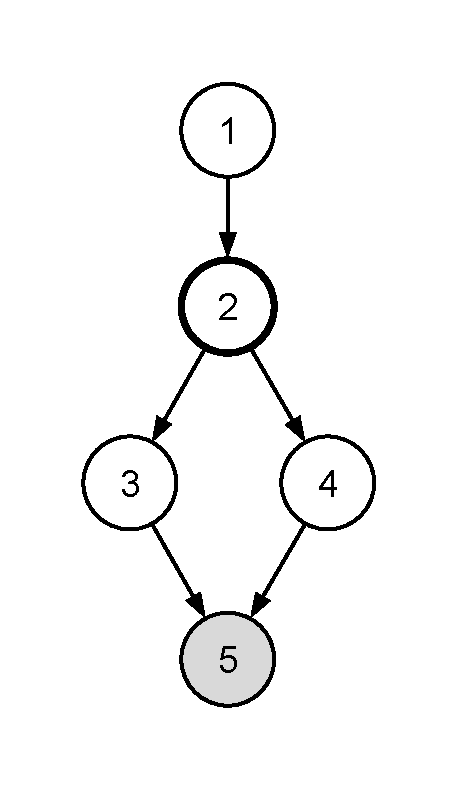
\includegraphics[width=0.3\linewidth]{fig01_simple_diamond/fig01_simple_diamond.pdf}
  \caption{The simple diamond. Source 1 feeds fork 2 (bold), whose two paths reconverge at join 5 (shaded).}
  \label{fig:pp-simple}
\end{figure}

The forward pass runs cleanly until the join. The fork's belief is the chain $b(2) = 1 \times 0.9 \times 0.9 = 0.81$, and each intermediate node follows as $b(3) = b(4) = 0.81 \times 0.9 \times 0.9 = 0.6561$, so each signal into the join carries $S = 0.6561 \times 0.9 = 0.59049$. Treating the two signals as independent, Eq.~\eqref{eq:pp-independent} gives
\[
b(5) \;=\; 0.9\,\bigl(1 - (1 - 0.59049)^2\bigr) \;=\; 0.749071 ,
\]
while exhaustive enumeration over all component states gives $b(5) = 0.675462$. The local update overestimates the join's belief by eleven per cent of its true value, and it does so because both signal events contain the fork's reachability. The two events are positively dependent, their intersection is larger than the product of their probabilities, and a union rule that understates the intersection overstates the union. On a network built deliberately out of redundancy the error is not a corner case but the norm, and it always flatters the system, reporting reliability the structure does not have.

Conditioning on the shared fork repairs the calculation. Given $R_2 = 1$ the two paths share nothing further, so each transmits independently with probability $0.9 \times 0.9 \times 0.9 = 0.729$ and the join receives a signal with probability $1 - (1 - 0.729)^2 = 0.926559$. Given $R_2 = 0$ nothing arrives, since every path into the join runs through the fork. Weighting the two cases by $P(R_2 = 1) = b(2) = 0.81$,
\[
P(\text{signal at } 5) \;=\; 0.81 \times 0.926559 \;=\; 0.750513 ,
\qquad
b(5) \;=\; 0.9 \times 0.750513 \;=\; 0.675462 ,
\]
the exact value. Two conditioned sub-problems replace an enumeration over $2^{10}$ component states, because conditioning is applied only to the one variable whose sharing created the dependence. That economy, exactness at the price of the dependence actually present, is the algorithm's entire design, and on real networks, where diamonds nest, overlap, and arrive several to a join, delivering it takes the machinery the diamond decomposition exists to provide.

\section{Conditioning at a Join}
\label{sec:pp-conditioning}

The example used two facts without naming them, that a belief can be split over the states of other nodes and that fixing the right node makes the parents' signals independent. A third governs the joins the example was too small to show, where several groups of parents arrive sharing nothing between them and each group's contribution must recombine with the others. All three hold in general, and together they justify the algorithm's treatment of any join. The structural objects come from Chapter~\ref{ch:diamond-module}, whose decomposition partitions each join's parents into groups of shared unfixed ancestry, anchors each group's diamond, and sets aside the non-influencing parents. A diamond arrives carrying its set $C$ of fixed nodes, and since the propagation resolves the diamond by conditioning on the reachability states of exactly those nodes, this chapter calls $C$ the \emph{conditioning set}.

\begin{lemma}[Conditional invariance]
\label{lem:pp-invariance}
For any set $A \subseteq V$ and any node $v$,
\[
b(v) \;=\; \sum_{c} P(R_A = c)\; P(R_v = 1 \mid R_A = c),
\]
where $R_A$ is the vector of reachability indicators of $A$ and the sum runs over its states $c \in \{0,1\}^{|A|}$. Every term is well defined because each $R_u$ is a deterministic function of the mutually independent component indicators.
\end{lemma}

\begin{proof}
The events $\{R_A = c\}$ partition the sample space, and the display is the law of total probability over that partition.
\end{proof}

\begin{lemma}[Separator sufficiency]
\label{lem:pp-separator}
Let $v$ be a join evaluated within a network in which every node of a fixed set $C$ enters only as a local source whose state is pinned, and suppose the influencing sets $\infl(u, C) = \anc(u) \setminus C$ of $v$'s parents within that network are pairwise disjoint. Then, conditional on $R_C = c$, the parents' signal events are mutually independent, and
\[
b(v \mid R_C = c) \;=\; \pi_v \Bigl( 1 - \prod_{u \in \Pa(v)} \bigl( 1 - P(R_u = 1 \mid R_C = c)\,\rho_{uv} \bigr) \Bigr).
\]
\end{lemma}

\begin{proof}
Every path into a parent $u$ either starts at a node of $C$, whose pinned state replaces everything upstream of it, or runs through components of $\infl(u, C)$ alone. Conditional on $R_C = c$, the signal event through $u$ is therefore a function of the constant $c$, of the indicators of the nodes of $\infl(u, C)$, of the edges among them, and of the edge $(u,v)$. The influencing sets are pairwise disjoint, so these indicator sets are pairwise disjoint and mutually independent, and functions of disjoint sets of independent variables are independent. The display is Eq.~\eqref{eq:pp-independent} applied conditionally.
\end{proof}

The hypotheses are not assumptions, because Chapter~\ref{ch:diamond-module} discharges both at every site where the propagation applies the independent update. Its edge isolation lemma guarantees that a fixed node appears in a diamond's edge list only as a local source, its outgoing edges kept and its upstream structure cut, and its grouping theorem certifies disjoint influencing sets, with the recursion extending the conditioning one covering fork at a time until the parents in view are disjoint in exactly this sense. The conditional beliefs the display consumes are the \emph{contextual beliefs}, the values each node holds within the sub-network currently being evaluated, which are conditional on the ambient states by construction because they were computed there.

The remaining question is the one Chapter~\ref{ch:diamond-module} deferred, whether the contributions of separately decomposed groups recombine correctly at the join. Its group disjointness theorem gives distinct groups pairwise disjoint influencing sets under the current context, and disjoint influence is exactly independence.

\begin{lemma}[Recombination across groups]
\label{lem:pp-recombination}
Fix a join $v$ and a context $E$ whose nodes' states are given, and let $G_1, \dots, G_m$ be the parent groups of the decomposition's partition at $v$, together with the singleton groups forming the non-influencing set. Write $E_k$ for the event that some parent in $G_k$ delivers a signal to $v$. The events $E_1, \dots, E_m$ are mutually independent, so
\[
P(\text{signal at } v) \;=\; 1 - \prod_{k=1}^{m} \bigl( 1 - P(E_k) \bigr),
\]
and each group is resolved on its own conditioning set alone.
\end{lemma}

\begin{proof}
Each $E_k$ is a function of the indicators of the nodes in $\bigcup_{p \in G_k} \infl(p, E)$, of the edges among them, and of the edges from $G_k$ into $v$. By group disjointness the node sets are pairwise disjoint, hence so are the edge sets they induce, and the given context enters every $E_k$ only as fixed constants. The events are therefore functions of pairwise disjoint sets of mutually independent indicators, hence mutually independent, and the display is the union rule for independent events.
\end{proof}

The lemma is also where the non-influencing set of Chapter~\ref{ch:diamond-module} earns its treatment. A non-influencing parent is a singleton group, its influencing set meeting no other's, so its signal enters the product as one more independent factor at the cost of a single multiplication, with no conditioning at all. A join can therefore gather several diamonds and several plain parents, and the recombination stays a one-line product over independent contributions.

Recombination across groups is where the decomposition pays for itself. A join whose $m$ groups carry conditioning sets $C_1, \dots, C_m$ is resolved in $\sum_k 2^{|C_k|}$ conditioned sub-problems, where conditioning on all the groups jointly would take $2^{\sum_k |C_k|}$. The gap is widest at high fan-in over independent structure. On an adversarial family in which $k$ independent reconvergent branches meet at one join, the implementation resolves exactly $2k + 1$ conditioned sub-problems for every $k$ tested up to $16$, linear where joint conditioning would be exponential.

What remains at a single group is the enumeration itself. Writing $C = \{a_1, \dots, a_m\}$ for the group's conditioning set, total probability gives
\begin{equation}
\label{eq:pp-enumeration}
P(E_k) \;=\; \sum_{c \,\in\, \{0,1\}^{m}} \; \Bigl( \prod_{i=1}^{m} \, b(a_i)^{c_i} \bigl(1 - b(a_i)\bigr)^{1 - c_i} \Bigr) \; \psi(c),
\end{equation}
where the weights are built from the conditioning nodes' contextual beliefs and $\psi(c)$ is the probability that the group delivers a signal to $v$ given the state $c$. A conditioning state does not simplify the diamond to a formula. It poses a smaller instance of the whole problem, and the algorithm answers it accordingly.

\section{Supernodes and Progressive Decomposition}
\label{sec:pp-supernodes}

A diamond arrives from Chapter~\ref{ch:diamond-module} as a graph object of the same form as the network itself, and the propagation exploits that self-similarity directly. For each state $c$ of the conditioning set, the algorithm poses the diamond as a network in its own right and runs on it the same single pass it runs on the whole. The local sources of that sub-network take their values from the enclosing computation, a conditioning node pinned to its state and every other local source keeping its contextual belief. The join's own prior is deferred, set to $1$ inside the sub-problem so that the sub-run returns the probability that a signal arrives, with the join's prior applied exactly once by the enclosing update. The value the sub-run returns at the join is $\psi(c)$.

The map $c \mapsto \psi(c)$ is all the enclosing computation ever needs from the diamond. Materialising that observation gives the algorithm its central reduction: the solved diamond is replaced by a \emph{supernode}, a single equivalent component that delivers a signal to the join with probability $\psi(c)$ under each state of its conditioning set.

\begin{lemma}[Supernode equivalence]
\label{lem:pp-supernode}
Let $D$ be a diamond at join $j$ with conditioning set $C$, solved in its context to the map $\psi_D$. Replacing $D$ by a supernode that delivers a signal to $j$ with probability $\psi_D(c)$ under each state $c$ leaves the belief of every node downstream of $j$ unchanged.
\end{lemma}

\begin{proof}
Fix a state $c$. Conditional on $R_C = c$, the event that $D$ delivers a signal to $j$ is a function of the indicators internal to $D$, which are independent of every indicator outside $D$. The enclosing computation only ever conditions on the nodes of its own conditioning sets, each of which enters the sub-network containing $D$ as a local source, upstream of $D$ or beside it, so each such conditioning event is a function of indicators outside $D$ and leaves $P(\text{signal at } j \mid R_C = c) = \psi_D(c)$ unchanged. A downstream belief depends on $D$ only through the signal event at $j$, entering by Lemma~\ref{lem:pp-invariance} as the pair of the weights $P(R_C = c)$ and the conditionals $\psi_D(c)$, and the supernode preserves both.
\end{proof}

The proof's independence step needs the enclosing computation to fix no node internal to $D$, and the decomposition guarantees exactly that. When an outer conditioning does reach inside a subgraph, the context-aware identity of Chapter~\ref{ch:diamond-module} makes the inner structure a different diamond with its own stored entry, so the sub-problem solved is always the one whose context actually holds.

Nesting makes the reduction progressive. Within a state's sub-run, an inner join with unresolved shared ancestry carries its own diamond, recorded by the decomposition in the enclosing diamond's substructure table, and the sub-run resolves it by the same conditioning, from the inside out. Termination is inherited from Chapter~\ref{ch:diamond-module}, whose recursion bounds the nesting by strictly growing the fixed context, and exactness follows by induction on nesting depth, each level applying Lemmas~\ref{lem:pp-invariance} to~\ref{lem:pp-supernode} within its own sub-network, which satisfies the same model assumptions as the whole.

Two mechanisms keep the recursion from repeating itself. A conditioned sub-problem is identified by its diamond's edge list together with the local source values its state assigns, and every solved sub-problem is stored under that identity, so a structurally identical sub-problem posed anywhere else in the recursion is answered from the store rather than recomputed. Separately, a conditioning node whose contextual belief is already pinned to $0$ or $1$ by the enclosing state carries no remaining uncertainty, so its enumeration collapses to the single state of non-zero weight. The collapse is exact because the discarded state has weight exactly $b\,{=}\,0$ or $1 - b\,{=}\,0$ in Eq.~\eqref{eq:pp-enumeration}.

\subsection{A multi-level worked example}
\label{sec:pp-worked}

The network of Figure~\ref{fig:pp-worked} exercises everything at once: three sources, three forks, nested diamonds, a join fed by a diamond and a non-influencing parent together, and a target whose reconvergence encloses every other structure. Sources $S_1$, $S_2$, $S_3$ have prior $1$, every other node prior $0.9$, and every edge probability $0.9$.

\begin{figure}[htbp]
  \centering
  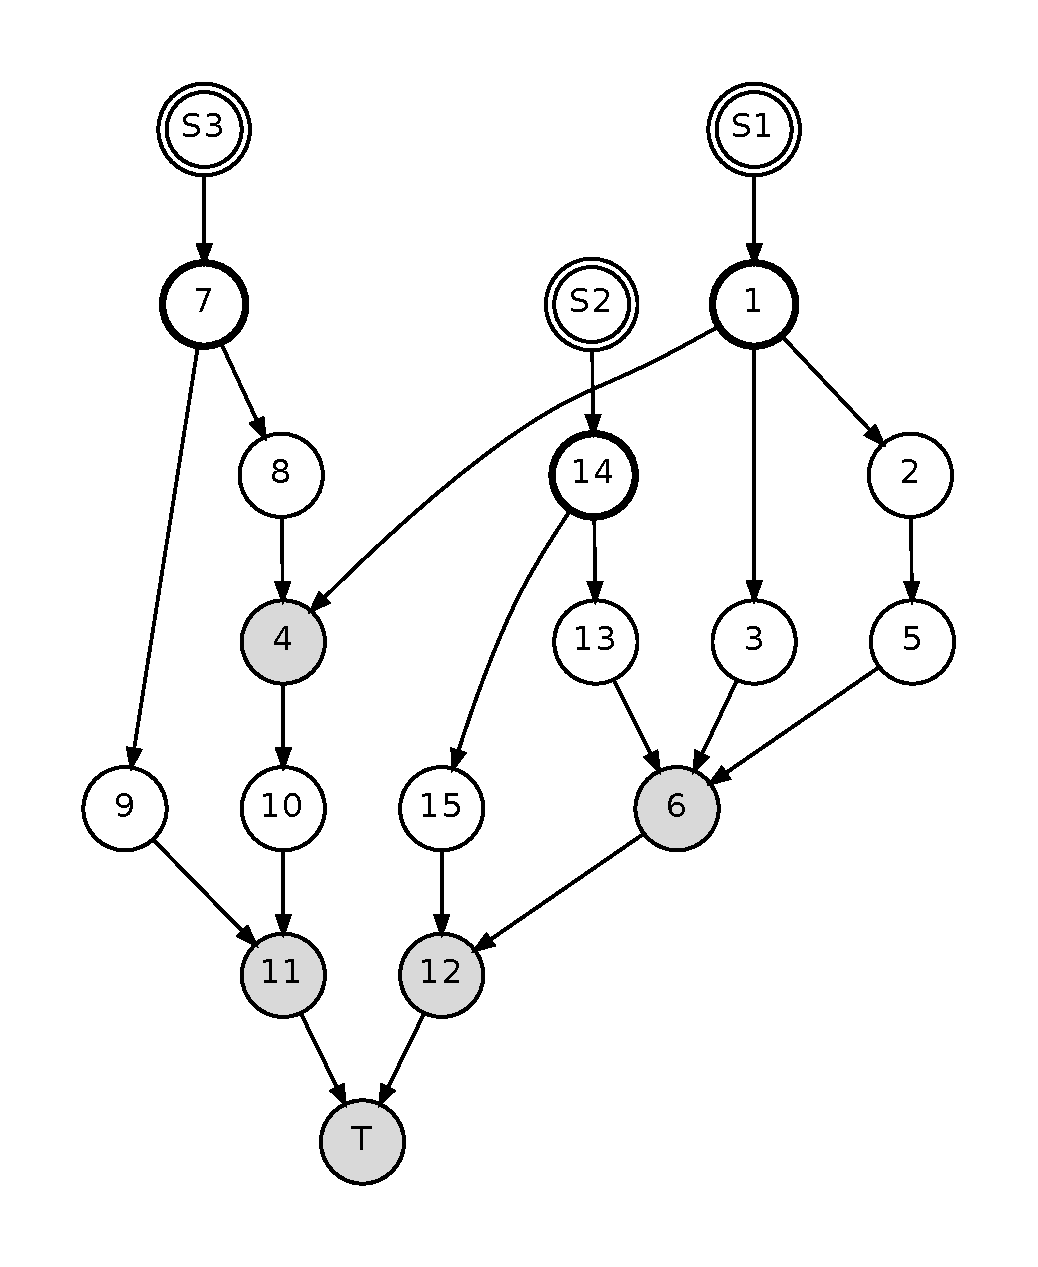
\includegraphics[width=0.5\linewidth]{fig03_worked_network/fig03_worked_network.pdf}
  \caption{The multi-level worked network. Sources are double-bordered, forks 1, 7 and 14 bold, joins 4, 6, 11, 12 and the target $T$ shaded.}
  \label{fig:pp-worked}
\end{figure}

The decomposition of Chapter~\ref{ch:diamond-module} returns four maximal diamonds. $D_1$ at join 6 anchors on fork 1, covering the reconvergent parents 5 and 3, while parent 13 arrives from $S_2$'s side sharing nothing with them and lands in the join's non-influencing set. $D_2$ at join 11 anchors on fork 7 and $D_3$ at join 12 on fork 14. $D_4$ at the target anchors on fork 1, because the target's two parents, 12 and 11, share exactly node 1 in their unfixed ancestry, and within $D_4$'s span the reconvergences at joins 11 and 12 recur as sub-diamonds. Join 4 receives parents 1 and 8 whose ancestries are disjoint, so it needs no diamond anywhere, and the plain update of Eq.~\eqref{eq:pp-independent} handles it at every level.

Table~\ref{tab:pp-trace} traces the four resolutions in the terms of Sections~\ref{sec:pp-conditioning} and~\ref{sec:pp-supernodes}. Each is a two-state enumeration whose weight is the conditioning node's contextual belief, here $0.81$ in all four cases since forks 1, 7 and 14 each sit one perfect source, one edge and one prior away.

\begin{table}[htbp]
\centering
\caption{Conditioning trace of the worked network. $w$ is the conditioning node's contextual belief, $\psi(1)$ and $\psi(0)$ the conditional signal probabilities the diamond's sub-runs return at the join, and $P(E)$ the group's recombined signal $w\,\psi(1) + (1-w)\,\psi(0)$.}
\label{tab:pp-trace}
\small
\renewcommand{\arraystretch}{1.2}
\begin{tabular}{lcccccc}
\toprule
Diamond & Join & $C$ & $w$ & $\psi(1)$ & $\psi(0)$ & $P(E)$ \\
\midrule
$D_1$ & 6  & $\{1\}$  & 0.81 & 0.889023 & 0        & 0.720108 \\
$D_2$ & 11 & $\{7\}$  & 0.81 & 0.893745 & 0.478297 & 0.814810 \\
$D_3$ & 12 & $\{14\}$ & 0.81 & 0.931860 & 0.583288 & 0.865631 \\
$D_4$ & $T$ & $\{1\}$ & 0.81 & 0.913943 & 0.818038 & 0.895721 \\
\bottomrule
\end{tabular}
\end{table}

At join 6 the diamond's contribution recombines with the non-influencing parent by Lemma~\ref{lem:pp-recombination}: parent 13 delivers its signal with probability $0.6561 \times 0.9 = 0.590490$ independently of the group, so the join receives a signal with probability $1 - (1 - 0.720108)(1 - 0.590490) = 0.885382$ and $b(6) = 0.9 \times 0.885382 = 0.796843$. The other three joins carry a single group each, so their beliefs follow directly from the table, $b(11) = 0.733329$, $b(12) = 0.779068$, and $b(T) = 0.806149$.

The dead states of $D_2$, $D_3$ and $D_4$ show why the conditioning is a genuine weighting rather than an on-off switch. With fork 7 down, join 11 is still reached through node 1's side at probability $0.478297$, with fork 14 down, join 12 is still reached through $S_1$'s side at $0.583288$, and with fork 1 down the target still collects the $S_2$ and $S_3$ routes at $0.818038$. Each of those values is itself the output of a full sub-network propagation in which the fork is a pinned local source, and inside $D_4$'s sub-runs the reconvergences at joins 11 and 12 are resolved by their own nested diamonds under the extended context.

The store is visible in the run, which poses twenty conditioned sub-problems of which sixteen are distinct. The four savings are the inner reconvergence at join 6, which $D_3$'s recursion meets again inside each of its states in exactly the form $D_1$ already solved, because node 14 lies outside that sub-problem's span, so the extended context is invisible to its identity and the store answers all four posings. The nested diamonds inside $D_4$ show the opposite case: node 1 lies inside their spans, its pinned state is part of their identity, and each is stored under both outer states, four entries apiece rather than two. The same subgraph is reused where the context cannot reach it and kept apart where it can, which is the context-aware identity of Chapter~\ref{ch:diamond-module} doing its work at propagation level. Every belief above agrees with exhaustive path enumeration under inclusion-exclusion to floating-point round-off.

\section{Validation}
\label{sec:pp-validation}

Every guarantee this chapter states has been checked against implementations that share none of the propagation's machinery. The exactness oracle is a reduced ordered binary decision diagram with dynamic variable reordering, built independently for each network, with exhaustive path enumeration where it is tractable and Monte Carlo estimation beyond. Across a corpus of 129 random and mutated DAGs, six topological families, larger random networks, and real and published benchmark networks, the propagated point beliefs agree with the oracle to a worst per-node deviation of $1.1 \times 10^{-16}$, under both perfect and imperfect component regimes. The propagated intervals coincide with the oracle's corner evaluations on all 129 graphs to at worst $2.8 \times 10^{-16}$, and the probability-box bounds were checked against Monte Carlo ground truth across fifty configurations spanning topology, input shape, and uncertainty width, with zero soundness violations. The measured cost of the corpus runs, alongside the oracle's, is the evidence base of the next section.

\section{Complexity Analysis}
\label{sec:pp-complexity}

The cost of the propagation is concentrated entirely in the diamonds, because everything outside them is the linear-time update of Eq.~\eqref{eq:pp-independent} applied once per node. A diamond with conditioning set $C$ and edge list $E_D$ is resolved by $2^{|C|}$ sub-runs, each a single pass over its edge list, so one resolution costs $2^{|C|} \cdot O(|E_D|)$, and the total work sums this over every sub-problem the recursion poses. The sum ranges over posings, not over unique diamonds. Nesting re-poses the same diamond under many enclosing states, as the worked example showed on a small scale, and on deeply nested networks the posing count exceeds the unique-diamond sum by orders of magnitude, so a budget computed over unique diamonds alone would understate the work.

Both refinements of Section~\ref{sec:pp-supernodes} act directly on this sum. The store collapses the posings to the genuinely distinct sub-problems, which across the validation corpus is between one and five per cent of the unmemoised posing bound, with the reduction factor a property of each network's nesting rather than a constant, so the posing bound is a sound a-priori budget, computable from the decomposition before any propagation runs, and the realised cost is typically far below it. The factorisation of Lemma~\ref{lem:pp-recombination} attacks the exponents themselves, replacing one joint enumeration by a sum of small ones, and its measured effect on the adversarial fan-in family, exactly $2k+1$ sub-problems against a joint $2^k$, is the difference between linear and exponential in the fan-in.

What no refinement removes is the width. The governing parameter is the largest conditioning set the network forces, and the algorithm's position among the exact methods of Section~\ref{sec:pp-survey} is fixed by it. The propagation is a specialisation of cutset conditioning \cite{pearl1988probabilistic} to source-to-node reachability, with two departures from the classical scheme. Where cutset conditioning selects one global set whose enumeration renders the whole network singly connected, the propagation identifies a local separator at each reconvergence actually encountered and recurses, so the realised cost is a sum of local exponentials rather than one global exponential, and tree-shaped regions are crossed at linear cost without touching any enumeration. And where the classical scheme conditions jointly, the factorisation refuses to enumerate independent forks together. Neither departure changes the complexity class. The largest conditioning set is bounded by the size of the largest set of mutually entangled shared ancestors, a quantity of the same nature as the treewidth that governs the junction tree \cite{lauritzen1988local} and the pathwidth that governs a well-ordered decision diagram \cite{bryant1986graph}, and all three methods are exponential in their width because \#P-hardness leaves no other shape available. No closed-form cost in the node count exists for any of them.

The measurements bear the placement out. Figure~\ref{fig:pp-width} plots the maximum conditioning set against the logarithm of the reordered decision diagram's node count across the corpus: the two track each other, seven against $\log_2 290 \approx 8.2$ on a published sixteen-node benchmark grid \cite{tong2019probability}, because both quantities measure the same structural width of the network. Realised work tells the same story with no winner. On some networks the propagation resolves fewer sub-problems than the diagram holds nodes and on others more, and no family in the corpus systematically favours either method for exact point-valued computation. Wall-clock comparisons move the crossover around without changing the conclusion. On a reconvergence-saturating adversarial family the propagation is faster up to moderate width and the diagram leads beyond it, on square meshes both grow exponentially with the diagram's exponent smaller, and on the fan-in family the propagation's linear sub-problem count wins outright. Where networks pass beyond the practical range, the two methods fail by different resources: on a reconvergence-dense Bayesian-network benchmark of 413 nodes and 265 joins, the decomposition's identification exhausts memory while the diagram's construction exhausts time, its reordering still compressing a diagram already past two and a half million nodes when the budget expires. Every exact method pays the width somewhere, and what differs is the resource and the point of failure.

\begin{figure}[htbp]
  \centering
  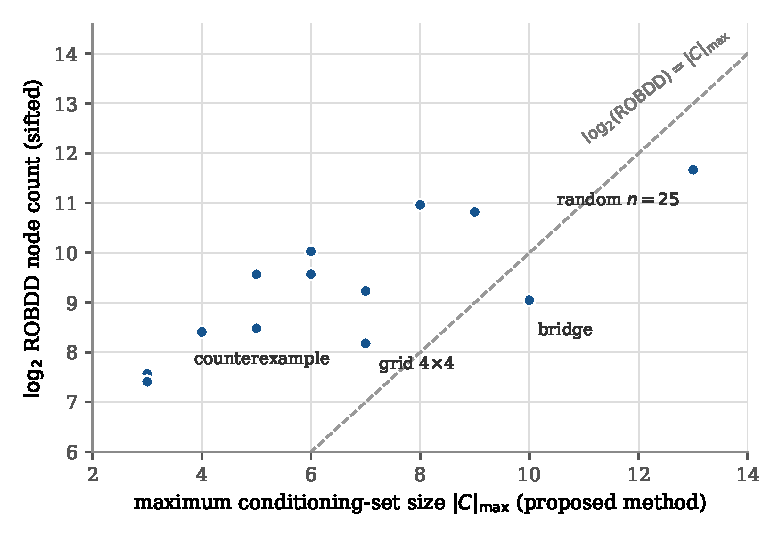
\includegraphics[width=0.72\linewidth]{fig04_width_correlation/width_correlation.pdf}
  \caption{Maximum conditioning-set size against the logarithm of the reordered decision diagram's node count across the complexity-validation networks. Both quantities measure the same structural width, and neither method dominates.}
  \label{fig:pp-width}
\end{figure}

The honest conclusion is that for exact point-valued reliability the propagation is competitive with a well-ordered decision diagram and not superior to it. Its case does not rest on a smaller state space. It rests on the two chapters of capability that follow, which decision diagrams do not offer at all.

\FloatBarrier

\section{Propagating Uncertain Probabilities}
\label{sec:pp-imprecise}

The inputs of a reliability analysis are rarely known exactly. Failure probabilities come from sparse operational records, manufacturer tolerances, and expert judgement, and Chapter~\ref{ch:system-model} gave the framework three value forms to carry those states of knowledge: a deterministic value asserting full knowledge, an interval asserting only bounds, and a probability box bounding a distribution. The usual fate of the honest forms is to be collapsed before the analysis begins, a point estimate chosen and the uncertainty deferred to an ad-hoc sensitivity study afterwards. The toolkit takes the opposite route and propagates the stated form itself, because everything the propagation does to a value is one of three operations, complement against one, product, and the weighted combinations of Eq.~\eqref{eq:pp-enumeration}, and none of the machinery of Sections~\ref{sec:pp-conditioning} and~\ref{sec:pp-supernodes} requires the values to be numbers. The framework realises the propagation once, generically, over all three forms. What is guaranteed of the output differs by form, and the next two sections establish the guarantee for each uncertain form in turn: the exact range for intervals, and sound distributional bounds for probability boxes.

\subsection{Interval inputs are propagated exactly}
\label{sec:pp-interval}

An interval input asserts that a component's reliability lies between two bounds and nothing more, and the correct output for a node is then the exact range of beliefs attainable over all inputs consistent with the stated bounds. The monotonicity of Section~\ref{sec:pp-belief} makes that range available outright.

\begin{proposition}[Corner exactness]
\label{prop:pp-corners}
Let every node prior and edge probability be given as an interval, $\pi_v \in [\underline{\pi}_v, \overline{\pi}_v]$ and $\rho_{uv} \in [\underline{\rho}_{uv}, \overline{\rho}_{uv}]$. The exact range of $b(v)$ over all inputs consistent with the intervals is
\[
\bigl[\, b(v)\ \text{at all lower endpoints},\;\; b(v)\ \text{at all upper endpoints} \,\bigr].
\]
\end{proposition}

\begin{proof}
By Proposition~\ref{prop:pp-monotone}, $b(v)$ is non-decreasing in every input coordinate, so over a box its minimum is attained where every coordinate sits at its lower endpoint and its maximum where every coordinate sits at its upper endpoint.
\end{proof}

No dependency problem arises and no corner search is needed, two consequences worth pausing on because neither is typical of interval computations. A general function over an input box takes its extremes at unknown corners among the $2^n$ available, and naive interval arithmetic on it over-approximates whenever a variable occurs more than once. Here monotonicity names the two extreme corners outright, and the propagation is arranged so that the arithmetic between them stays exact. Its complement and product are exact interval operations, the product form of Eq.~\eqref{eq:pp-independent} presents each signal to the arithmetic exactly once, and the conditioning combination is evaluated at the endpoint values of each conditioning belief, which suffices because Eq.~\eqref{eq:pp-enumeration} is multilinear in each of them and a multilinear function attains its extremes over a box at its corners. Every step returns an enclosure of the true range, and across the full validation corpus the propagated interval coincides with the two corner propagations to machine precision, at worst $2.8 \times 10^{-16}$ in either bound over all 129 graphs. On the worked network with every non-source prior and every edge widened to $[0.85, 0.95]$, the propagated belief at the target is $[0.634002, 0.931254]$ and agrees with the two corner runs exactly, to the last floating-point digit. Structural certainties are kept degenerate in such a widening, a perfect source stays $[1,1]$, because degrading a certainty into an uncertainty does not perturb the problem, it changes which nodes can carry conditioning and poses a different and harder one.

The conditioning machinery matters as much here as for point values. An interval propagation that ignores reconvergent dependence stays sound but over-widens, by up to $0.45$ of the unit range on the corpus, wide enough to turn an informative bound into a vacuous one. Exactness of the range is a property of conditioning, not of interval arithmetic alone.

Carrying intervals is nearly free. The propagation costs a factor of about $1.2$ over point propagation, a few extra floating-point operations per step, and for a one-shot query, producing a network's belief range from scratch, it completed faster than the decision-diagram route to the same range, building the diagram once and evaluating its two corners, on every one of eight corpus families tested, by factors between $3.9$ and $99.9$. The claim is scoped to the one-shot cost, where the diagram's construction counts against it, and a workload that amortises one diagram across many repeated queries on a fixed network is a different and untested scenario.

\section{Probability-Box Propagation}
\label{sec:pp-pbox}

A probability box is the strongest of the three input forms, a pair of bounding distribution functions carrying partial statistical knowledge of an uncertain reliability \cite{ferson2003constructing}, and propagating it promises the strongest output: bounds on the entire distribution of a node's belief, from which any decision quantity over that distribution can be bounded in turn. The promise comes with one genuinely new mathematical difficulty, and this section locates it, resolves it, and is explicit about what is proved and what is not.

\subsection{The conditioning combination is not a convolution}
\label{sec:pp-pbox-operator}

The chain and union steps of the propagation raise no new issue for distributional values, because the quantities they combine are independent by the same structural discipline that makes the point computation exact, and p-box arithmetic under independence is standard \cite{williamson1990probabilistic}. The difficulty sits exactly at the conditioning combination. Taking the conditioning nodes one at a time, Eq.~\eqref{eq:pp-enumeration} is the convex combination
\[
W \cdot A + (1 - W) \cdot B ,
\]
where $W$ is the conditioning node's contextual belief and $A$, $B$ the conditional results of its two states. All three are now uncertain quantities, and two dependencies bind them. $A$ and $B$ are functions of the same upstream reliabilities, so they are dependent on each other, and the two coefficients are one random variable, not two. Convolving the terms as if independent ignores both bindings, and the consequence is not mild conservatism but unsoundness: probability mass escapes the unit interval, by as much as $0.34$ on the benchmark grid of Section~\ref{sec:pp-complexity}. A distributional result that assigns mass outside $[0,1]$ bounds nothing, so the operator has to respect the combination's structure.

The framework's operator integrates over the weight's own uncertainty. At each discretisation level of $W$'s bounding functions it scales the two branch distributions by $w$ and $1 - w$ and combines them under an explicit bound on their dependence, mixes the results across levels, and envelopes the mixture built on $W$'s lower bounding function with that built on its upper. Applied one conditioning node at a time, the nested two-way combination reproduces the full mixture over all $2^{|C|}$ states. The output is finally intersected with $[0, 1]$, a projection that discards only values a probability cannot take and so can tighten but never invalidate a bound, and the projection is guarded, raising an error rather than clipping silently if the excursion ever exceeds floating-point round-off by orders of magnitude, so that a genuine soundness regression can never hide inside the projection.

\subsection{Two dependence bounds, one proved and one open}
\label{sec:pp-pbox-blends}

The dependence bound between the branches is where provability and tightness part company, and the two must not be conflated with each other or with soundness itself. Sound means the computed pair of bounding functions contains the true distribution, and a sound result is never wrong. Tight means the pair is narrow, and a sound result can still be too wide to use. The choice of bound trades one against the other.

Bounding the branches by the Fr\'echet--Hoeffding inequalities is valid under any joint dependence whatsoever, so the resulting belief bounds inherit soundness from a classical theorem \cite{williamson1990probabilistic} with no proof burden here, at the price of width, and on hard cases the width can approach vacuity. The framework's default blend instead restricts the dependence bound to non-negative dependence, on the ground that $A$ and $B$ are both non-decreasing functions of the shared upstream reliabilities and so cannot move against each other. The restricted blend is tighter and never vacuous in practice, and it has produced no soundness violation in any of the fifty validation configurations checked against Monte Carlo ground truth. But the motivating argument is not a proof. The dependence-bound literature offers a strict trichotomy, independence, a fully specified dependence, or no assumption at all, with no theorem for positive-but-otherwise-unknown dependence, and an attempted derivation through the natural ordering-of-dependence route meets a genuine obstruction rather than a technicality. Soundness of the restricted blend therefore stands as an open question, stated as such, and the framework keeps the distinction operational: the restricted blend is the default, and the Fr\'echet blend is used wherever a claim must rest on proof alone.

\subsection{What the bounds are worth}
\label{sec:pp-pbox-value}

Soundness never varies across the validation sweep, and tightness does, so the honest characterisation of the output is an envelope rather than a single figure. Figure~\ref{fig:pp-envelope} sweeps input-distribution shapes, uncertainty widths, and reconvergence regimes on the benchmark grid: the bound band is near $0.18$ of the unit range under high component reliability and weak reconvergence, degrades to about $0.70$ under deep reconvergence with broadly uncertain components, and is driven by the regime and the input width rather than by the shape of the input distributions, with zero violations anywhere in the sweep. Deep reconvergence under broad uncertainty is precisely where the branch dependence is strongest and any distribution-free bound on it loosest, so the envelope's shape is the mathematics showing through, not an artefact to engineer away.

\begin{figure}[htbp]
  \centering
  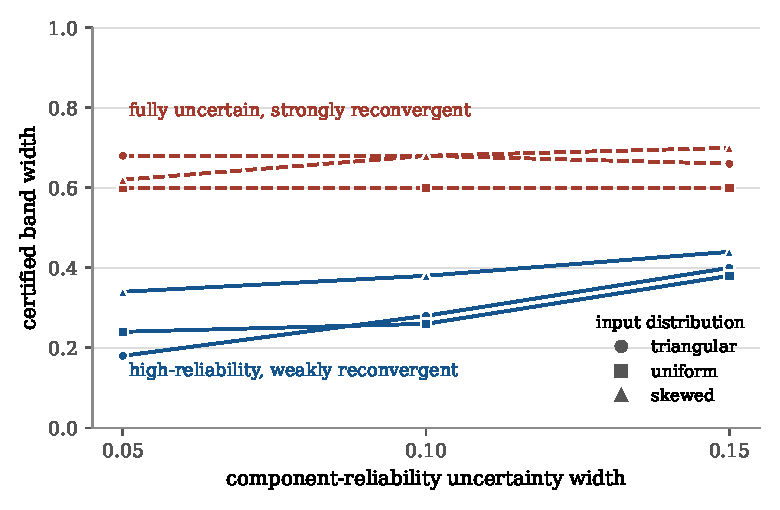
\includegraphics[width=0.78\linewidth]{fig05_envelope/envelope.pdf}
  \caption{Tightness envelope of the propagated probability-box bound on the benchmark grid: band width against component uncertainty width, across input-distribution shapes and reconvergence regimes. Soundness holds in every configuration, and only tightness varies, driven by regime and width rather than input shape.}
  \label{fig:pp-envelope}
\end{figure}

The practical payoff is a certificate no point-valued exact method produces. The output bounds the distribution of $b(v)$, so for a stated reliability requirement $x^{\ast}$ it bounds $P(b(v) \le x^{\ast})$, the probability that the node fails its requirement, analytically and from a single propagation. Table~\ref{tab:pp-certified} shows the certified band on that probability at a representative requirement of $x^{\ast} = 0.95$ on the benchmark grid, between $0.02$ and $0.12$ wide across the regimes tested. Matching that precision by simulation, planned conservatively without foreknowledge of the answer, costs between $267$ and $9{,}604$ samples of the network's uncertain inputs, and the result remains a statistical estimate rather than a bound. The planning figure is the honest one to quote, because the retrospective sample requirement collapses whenever the true probability sits near $0$ or $1$, correct statistics but knowable only in hindsight. A decision diagram has no analytic route to this quantity at all and would itself fall back on simulation.

\begin{table}[htbp]
\centering
\caption{Certified bound on the requirement-violation probability $P(b(v) \le 0.95)$ at the benchmark grid's target node, from one propagation, against the Monte Carlo sample count required to match the certified precision under worst-case a-priori planning.}
\label{tab:pp-certified}
\small
\renewcommand{\arraystretch}{1.2}
\begin{tabular}{llccc}
\toprule
Regime & Uncertainty width & Certified band & Band width & MC samples \\
\midrule
perfect components & 0.05 & $[0.00,\, 0.02]$ & 0.02 & 9{,}604 \\
perfect components & 0.10 & $[0.00,\, 0.10]$ & 0.10 & 385 \\
perfect components & 0.15 & $[0.00,\, 0.12]$ & 0.12 & 267 \\
uncertain components & 0.05--0.15 & $[0.98,\, 1.00]$ & 0.02 & 9{,}604 \\
\bottomrule
\end{tabular}
\end{table}

\subsection{The cost of the distribution}
\label{sec:pp-pbox-cost}

Distributional propagation is not cheap and is not claimed to be. Its cost is a dial, the discretisation level of the bounding functions, and grows roughly cubically with it, measured at $1.2$, $6.0$, $39$ and $276$ seconds at levels $25$, $50$, $100$ and $200$ on a fifteen-node reference network, in exchange for proportionally tighter bands. The bounds are sound at every level, so the level buys precision, never correctness, and levels between $25$ and $100$ are the practical band on networks of the scale the exact method suits. The conditioning depth itself is unchanged across all three value forms, so imprecision never relaxes the structural cost of Section~\ref{sec:pp-complexity}, and a network too reconvergent for exact point propagation is equally beyond exact interval or distributional propagation. Where a network supports exact propagation but not the distributional dial, the exact interval range together with sampling is the practical recourse.

\section{Case Study: A Medical Drone Logistics Network}
\label{sec:pp-case}

The capabilities of this chapter come together on a real planning problem. Jones et al.\ designed a conceptual medical drone delivery network for Scotland \cite{jones2025conceptual}, optimising station placement and network structure over real hospital, airport, and candidate-station locations, with two drone types, a short-range vertical take-off type with a nominal range of 70~km and a long-range fixed-wing type with a nominal range of 700~km, trading off delivery time, capital cost, and resilience. Their own resilience analysis works with point probabilities. The question their framework structurally cannot answer, and this toolkit can, is how confidently each location in a candidate design can be called reachable from the supply hubs once the acknowledged uncertainty in the component availabilities is carried honestly through the network.

\subsection{Inputs, traced to their source}
\label{sec:pp-case-inputs}

Every input of the reliability model derives from the source study, with one clearly flagged extension. Location availability follows the study's own resilience assumption, hub locations always available and every other location failing independently with probability $0.2$. The hub availability is kept at exactly $1$, and the non-hub availability becomes the interval $[0.75, 0.85]$ centred on the study's figure, a deliberate choice because that figure is stated as an assumption rather than derived from data, and an interval input turns the whole analysis into a built-in sensitivity assessment of precisely that assumption. A connection exists, per drone type, exactly when the inter-location distance is within the type's stated nominal range, the study's own construction rule applied unchanged, and where both types serve a connection the two transmissions combine as independent alternatives.

The flagged extension concerns weather. The source study holds wind conditions constant in its own analysis and defers weather-driven range variation as an uncertainty that would need expert elicitation. The reliability model extends exactly that deferred point and nothing else: a connection operating comfortably within a drone's range is treated as reliable, and a connection whose length falls in the final ten per cent of the range, an illustrative derating margin since the study quantifies none either, receives the vacuous interval $[0,1]$, the honest statement that adverse weather may or may not close that particular route. Direction, finally, follows the supply logic. The study's connections are undirected because a route can be flown either way, but the reliability question concerns supply reaching facilities from hubs, so the dependency graph is directed from the hub tier outward, matching the study's own hub-and-spoke architecture.

\subsection{Three designs and the redundancy boundary}
\label{sec:pp-case-designs}

The study's actual optimised layouts are not published, so three configurations stand as proxies for the qualitative character of three of its described trade-off points: a fixed-wing-reliant centralised design serving remote locations through a hub backbone, 217 locations and 263 connections, a densely interconnected short-range design, 242 locations and 1{,}753 connections, and a minimal-investment design retaining only pre-existing infrastructure, 230 locations and 1{,}648 connections. They are proxies for a described character, not reproductions of an unavailable result, and every conclusion below attaches to them as such.

Constructing the dense designs runs directly into the boundary this chapter has been pricing. Connecting every operationally plausible pair of locations produces a network whose identification alone did not complete, exhausting the memory of the analysis machine within minutes, so unrestricted connectivity sits beyond the practical range of exact analysis outright. The design parameter that controls the boundary is a genuine engineering quantity, the number of alternate routes provisioned per location, a redundancy choice and not a parameter of the method. Provisioning sixteen routes per location brings the conditioning width of the dense designs to 16 and 17, deliberately just inside the practical ceiling of around eighteen that earlier experience with the method located, and provisioning beyond sixteen changes neither the width nor the runtime materially, so the reconvergent structure of this network saturates there. The centralised design, tree-like by construction, carries width 10. Full exact interval propagation completes in under 25 seconds on the dense designs and well under a second on the centralised one.

The same boundary was measured for the decision-diagram alternative on the same networks, with identical inputs, and the two methods agree to floating-point precision everywhere both complete. At low redundancy both are comfortably fast, and the one-shot interval computation of the propagation is faster, by roughly a factor of fifty on the centralised design and fifteen on the minimal design provisioned at six routes. Raising the provision, the diagram construction completes up to twelve routes per location, at a build of some 123{,}000 nodes in 45 seconds, and did not complete within a documented budget from fourteen routes, under dynamic reordering, while the propagation's runtime stays near five seconds across the same sweep. The claim this supports is deliberately narrow. Both methods are governed by the same structural width, and on this one real network family the propagation's practical range, measured along a real redundancy parameter, extends further than the diagram's, with the crossover bracketed between twelve and fourteen routes rather than located.

Distributional propagation has its own, tighter boundary on the same family, exactly as Section~\ref{sec:pp-pbox-cost} prices it. The full probability-box analysis completes in seconds on the centralised design and in minutes on the minimal design provisioned at six routes, and at eight routes it did not complete within an hour, so the distributional dial is affordable precisely on the sparser designs, and interval propagation, exact and near-free, is what scales to the dense ones.

\subsection{What the propagated bounds say}
\label{sec:pp-case-results}

Table~\ref{tab:pp-drone} collects the propagated reliability bounds, and they are informative in exactly the way the designs differ. In the centralised design every location's band is narrow, at most $0.10$ wide with a mean of $0.089$: reachability essentially inherits the availability band assumed for the locations themselves, because a tree accumulates little dependence, but it also enjoys no protection, since any single-route failure disconnects service outright. The dense designs spread. Well-connected locations are reachable with near-certainty, and the worst-served facility, Islay Hospital, an island site, carries a reachability probability bounded between $0.56$ and $0.72$ in both dense designs. That interval is the honest answer to the planning question under the acknowledged input uncertainty, and it is a different kind of answer than a point analysis can give: a facility whose reachability is confidently $0.6$ and one whose reachability is anywhere between $0.56$ and $0.72$ call for different interventions, better routes for the first, better component data before committing capital for the second, and no point-valued analysis of the same design can tell them apart. Figure~\ref{fig:pp-dronemap} maps the dense decentralised design coloured by the lower reliability bound and by band width. The uncertainty concentrates at island and far-northern facilities, which is where additional redundancy, or better availability data, buys the most, and the map is the toolkit's output translated back onto the geography the source study planned over.

\begin{table}[htbp]
\centering
\caption{The three proxy designs: structure, conditioning width, and propagated interval reliability bounds. Every belief is contained in $[0,1]$ with lower bound at most upper bound. The worst-served facility in both dense designs is Islay Hospital.}
\label{tab:pp-drone}
\small
\renewcommand{\arraystretch}{1.2}
\begin{tabular}{lrrrccc}
\toprule
Design & $|V|$ & $|E|$ & width & mean band & max band & worst facility \\
\midrule
fixed-wing centralised & 217 & 263 & 10 & 0.089 & 0.100 & $[0.750,\, 0.850]$ \\
dense decentralised & 242 & 1753 & 17 & 0.094 & 0.161 & $[0.562,\, 0.722]$ \\
concentrated minimal & 230 & 1648 & 16 & 0.093 & 0.161 & $[0.562,\, 0.722]$ \\
\bottomrule
\end{tabular}
\end{table}

\begin{figure}[htbp]
  \centering
  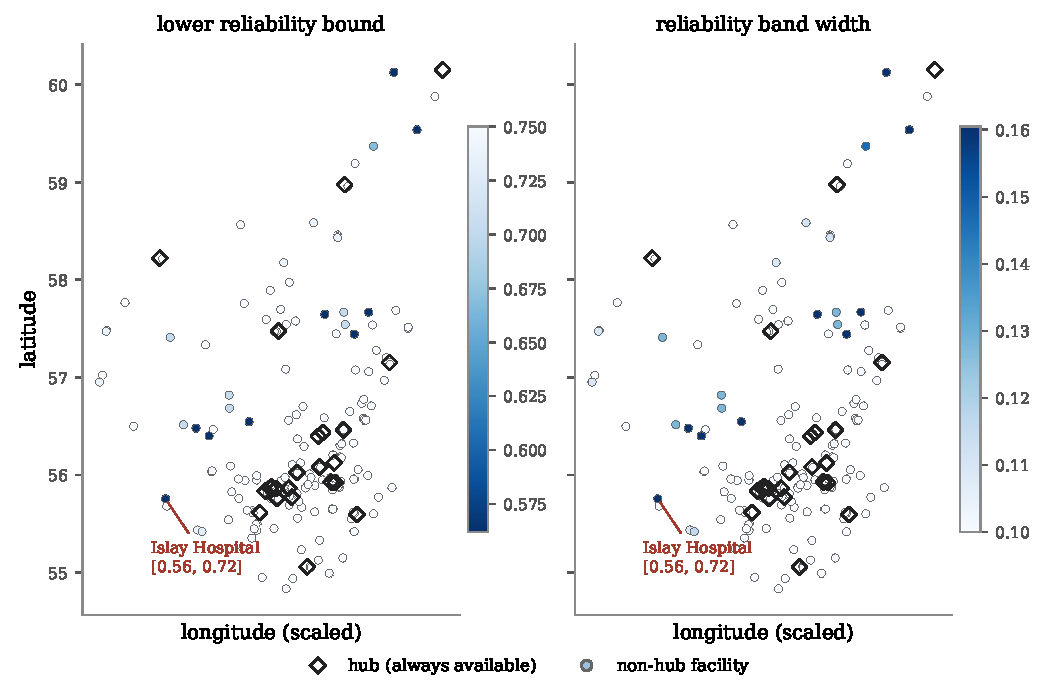
\includegraphics[width=\linewidth]{fig06_drone_map/drone_reliability_map.pdf}
  \caption{Reliability map of the dense decentralised design: each facility coloured by the lower bound of its propagated reachability (left, darker is less certainly reachable) and by the width of its reliability band (right, darker is more uncertain). Hubs, drawn as diamonds, are assumed always available. Uncertainty concentrates at island and far-northern facilities, and the worst-served facility, Islay Hospital, is bounded at $[0.56, 0.72]$.}
  \label{fig:pp-dronemap}
\end{figure}

The case study also returns something to the design process itself. More provisioned redundancy improves resilience and simultaneously raises the cost of verifying it exactly, and on this network that trade-off is now a measured curve rather than a caution: the width saturates at sixteen routes per location, exact verification is practical there, and the point at which the alternative exact method stops being practical sits measurably earlier. A designer choosing between these configurations can see, in the same analysis, which facilities are uncertain, why they are uncertain, and what verifying a more redundant design will cost.

\section{Summary}
\label{sec:pp-summary}

The toolkit computes the belief of every node, the probability that it operates and is reached from a source, in one pass over the layered order, applying the closed-form update wherever parent signals are independent and resolving every reconvergence by conditional enumeration on the diamonds of Chapter~\ref{ch:diamond-module}. Lemmas~\ref{lem:pp-invariance} to~\ref{lem:pp-supernode} carry the exactness argument: total probability splits a belief over conditioning states, the diamond's fixed nodes make parents conditionally independent, disjoint groups recombine by the independent union, and a solved diamond stands in for its subgraph as a supernode, which discharges the two claims Chapter~\ref{ch:diamond-module} deferred to this chapter. The cost is exponential only in the conditioning width the network forces, the same parameter that governs cutset conditioning, junction trees, and well-ordered decision diagrams, and for point-valued inputs the method is competitive with, not superior to, that established class. Its distinctive capability is that the same propagation carries the framework's uncertain value forms natively, returning the exact belief range for interval inputs by monotonicity, and guaranteed distribution bounds for probability-box inputs through a conditioning operator built on the Fr\'echet--Hoeffding inequalities, certifying decision-relevant probabilities from a single propagation. On a real medical logistics network those capabilities produce what the chapter set out to produce, an honest reliability map under acknowledged input uncertainty, and a measured account of what exactness costs and where it ends.

\ifdefined\maindoc
% do nothing
\else
\printbibliography
\end{document}
\fi
